\section{Affine $n$-Space and Algebraic Sets}

\begin{definition}
    Let $k$ be a field. We define  \textbf{affine $n$-space} over $k$ to be the
    cartesian product  $\A^n(k) = \underbrace{k \times \dots \times
    k}_{n\text{-times}}$. If the field $k$ is understood, we write  $\A^n$. We
    call the elements of  $\A^(k)$ \textbf{affine points}. We call $\A^1(k)$ and
    $\A^2(k)$ the \textbf{affine line} and \textbf{affine plane} over $k$,
    respectively.
\end{definition}

\begin{definition}
    Let $k$ be a field, and let  $f \in k[x_1, \dots, x_n]$. We call an affine
    point $P \in \A^n(k)$ a \textbf{zero}, or \textbf{root} of $f$ if $f(P)=0$,
    where $f(P)$ is understood to be $f(a_1, \dots, a_n)$, where $P=(a_1, \dots,
    a_n)$. We call the set of zeros of $f$, $V(f)$ the \textbf{hypersurface}
    defined by $f$. We call hypersurfaces in  $\A^2(k)$ \textbf{affine plane
    curves}. If $\deg{f}=1$, we call $V(f)$ a \textbf{hyperplane}. We call
    hypersurfaces in $\A^1(k)$ \textbf{lines}.
\end{definition}

\begin{example}\label{example_2.1}
    The following are algebraic curves.
    \begin{figure}[h]
        \centering
        \includegraphics[scale=0.5]{Figures/Chapter1/hyperplanes.svg}
        \caption{}
        \label{}
    \end{figure}
\end{example}

\begin{definition}
    Let $k$ be a field, and $S$ any set of polynomials in $k[x_1, \dots, x_n]$.
    We define the \textbf{set of zeros} of $S$ to be the set  $V(S)=\{P \in
    \A^n(k) : f(P)=0 \text{ for all } f \in S\}$. We call a subset $X$ of
    $\A^n(k)$ an \textbf{affine algebraic set} if $X=V(S)$ for some set $S$ of
    polynomials.
\end{definition}

\begin{lemma}\label{1.2.1}
    The following are true for any field $k$.
    \begin{enumerate}
        \item[(1)] If $\af$ is an ideal in $k=[x_1, \dots, x_n]$ generated by a
            set $S \subseteq k[x_1, \dots, x_n]$, then $V(\af)=V(S)$.

        \item[(2)] If $\{\af_\a\}$ is a collection of ideals of $k[x_1, \dots,
            x_n]$, then
            \begin{equation*}
                V\Big{(} \bigcup{V(\af_\a)} \Big{)}=\bigcap{V(\af_\a)}
            \end{equation*}

        \item[(3)] If $\af \subseteq \bf$ are idelas, then  $V(\bf) \subseteq
            V(\af)$.

        \item[(4)] If $f,g \in k[x_1, \dots, x_n]$, then $V(fg)=V(f) \cup V(g)$.

        \item[(5)] $V(0)=\A^n(k)$ and $V(1)=\emptyset$.
    \end{enumerate}
\end{lemma}
\begin{proof}
\end{proof}
